%%%%%%%%%%%%%%%%%%%%%%%%%%%%%%%%%%%%%%%%%
% Beamer Presentation
% LaTeX Template
% Version 1.0 (10/11/12)
%
% This template has been downloaded from:
% http://www.LaTeXTemplates.com
%
% License:
% CC BY-NC-SA 3.0 (http://creativecommons.org/licenses/by-nc-sa/3.0/)
%
%%%%%%%%%%%%%%%%%%%%%%%%%%%%%%%%%%%%%%%%%

%----------------------------------------------------------------------------------------
%	PACKAGES AND THEMES
%----------------------------------------------------------------------------------------
\documentclass[aspectratio=169]{beamer}

\mode<presentation> {

% The Beamer class comes with a number of default slide themes
% which change the colors and layouts of slides. Below this is a list
% of all the themes, uncomment each in turn to see what they look like.

%\usetheme{default}
%\usetheme{AnnArbor}
%\usetheme{Antibes}
%\usetheme{Bergen}
%\usetheme{Berkeley}
%\usetheme{Berlin}
%\usetheme{Boadilla}
%\usetheme{CambridgeUS}
%\usetheme{Copenhagen}
%\usetheme{Darmstadt}
%\usetheme{Dresden}
%\usetheme{Frankfurt}
%\usetheme{Goettingen}
%\usetheme{Hannover}
%\usetheme{Ilmenau}
%\usetheme{JuanLesPins}
%\usetheme{Luebeck}
\usetheme{Madrid}
%\usetheme{Malmoe}
%\usetheme{Marburg}
%\usetheme{Montpellier}
%\usetheme{PaloAlto}
%\usetheme{Pittsburgh}
%\usetheme{Rochester}
%\usetheme{Singapore}
%\usetheme{Szeged}
%\usetheme{Warsaw}

% As well as themes, the Beamer class has a number of color themes
% for any slide theme. Uncomment each of these in turn to see how it
% changes the colors of your current slide theme.

%\usecolortheme{albatross}
%\usecolortheme{beaver}
%\usecolortheme{beetle}
%\usecolortheme{crane}
%\usecolortheme{dolphin}
%\usecolortheme{dove}
%\usecolortheme{fly}
%\usecolortheme{lily}
%\usecolortheme{orchid}
%\usecolortheme{rose}
%\usecolortheme{seagull}
%\usecolortheme{seahorse}
%\usecolortheme{whale}
%\usecolortheme{wolverine}

%\setbeamertemplate{footline} % To remove the footer line in all slides uncomment this line
\setbeamertemplate{footline}[frame number] % To replace the footer line in all slides with a simple slide count uncomment this line


\setbeamertemplate{navigation symbols}{} % To remove the navigation symbols from the bottom of all slides uncomment this line
}

% \usepackage[style=authoryear]{biblatex}
\usepackage{biblatex}
\usepackage{graphicx} % Allows including images
\usepackage{booktabs} % Allows the use of \toprule, \midrule and \bottomrule in tables
%\usepackage {tikz}
\usepackage{tkz-graph}
\GraphInit[vstyle = Shade]
\tikzset{
  LabelStyle/.style = { rectangle, rounded corners, draw,
                        minimum width = 2em, fill = yellow!50,
                        text = red, font = \bfseries },
  VertexStyle/.append style = { inner sep=5pt,
                                font = \normalsize\bfseries},
  EdgeStyle/.append style = {->, bend left} }
\usetikzlibrary {positioning}
%\usepackage {xcolor}
\definecolor {processblue}{cmyk}{0.96,0,0,0}


% My macros
\usepackage{lipsum}
\usepackage{caption}

\newcommand{\backupbegin}{
   \newcounter{finalframe}
   \setcounter{finalframe}{\value{framenumber}}
}
\newcommand{\backupend}{
   \setcounter{framenumber}{\value{finalframe}}
}


\newcommand\blfootnote[1]{%
  \begingroup
  \renewcommand\thefootnote{}\footnote{#1}%
  \addtocounter{footnote}{-1}%
  \endgroup
}
\def\trainingset{\{x_i,y_i\}_{i=1}^{N}}
\def\pNMLSingle{p_{\hat{\theta}(z^N,x,y)} (y|x)}
\newcommand{\SubItem}[1]{
    {\setlength\itemindent{15pt} \item[-] #1}
}
\usepackage{amsmath}
\DeclareMathOperator*{\argmax}{arg\,max}
\DeclareMathOperator*{\argmin}{arg\,min}
\newcommand\tableref{Table~\ref}
\def\Dc{\mathcal{D}_c}
\def\Du{\mathcal{D}_u}
\newcommand\cC{{\cal C}}
\newcommand{\minisection}[1]{\vspace{2mm}\noindent{\textbf{#1.}}}
\newcommand\koby[1]{\textcolor{blue}{[KB: #1]}}
\newcommand\meir[1]{\textcolor{red}{[MF: #1]}}
\newcommand{\ignore}[1]{}

%----------------------------------------------------------------------------------------
%	TITLE PAGE
%----------------------------------------------------------------------------------------

\title[Short title]{Universal Learning of Individual Data} % The short title appears at the bottom of every slide, the full title is only on the title page


\date{September 2020} % Date, can be changed to a custom date

\subtitle{Ph.D. Research Proposal}
\author[]{\fontsize{12}{14}\selectfont Koby Bibas \\ \vspace{3pt}
Advisor: Prof.~Meir~Feder}

\institute[\large Tel Aviv University]
{
\includegraphics[scale=0.075]{TAU-NEW-LOGO.jpg}} 

\bibliography{references.bib}
\begin{document}

\begin{frame}
\titlepage % Print the title page as the first slide
\end{frame}

% \begin{frame}
% \frametitle{Overview} % Table of contents slide, comment this block out to remove it
% \tableofcontents % Throughout your presentation, if you choose to use \section{} and \subsection{} commands, these will automatically be printed on this slide as an overview of your presentation
% \end{frame}

%--------------------------------------------------
%	PRESENTATION SLIDES
%--------------------------------------------------
\begin{frame}{Outline}
\tableofcontents
\end{frame}



% ------------------------------ %
\section{Introduction}
% ------------------------------ %
\begin{frame}[c]
\begin{center}
\Huge Introduction
\end{center}
\end{frame}



\subsection{The supervised learning setting}
\begin{frame}{The supervised learning setting}
\begin{itemize}
\setlength\itemsep{1.5em}
\item A trainset $z^N = \{(x_i,y_i)\}_{i=1}^N$ is given. 
\item The goal is to predict the label $y$ of test data $x$. 
\item We assume to have a model class $\Theta$.
\item A predictor $q_{\theta}(\cdot|x) \ \theta \in \Theta$, is evaluates using the log-loss  
    \begin{equation*}
    \mathcal{L}(q_\theta, x, y) = -\log {q_\theta(y|x}).
    \end{equation*}
\item The Empirical Maximum Likelihood (ERM) learner
\begin{equation}
    \theta_{ERM} = \argmin_{\theta \in \Theta} \sum_{i=1}^N \mathcal{L}(q_\theta, x_i, y_i)
\end{equation}
\end{itemize}
\end{frame}



\begin{frame}{Learning of individual data}
\begin{itemize}
\setlength\itemsep{0.5em}
\item Individual Settings $x,y \not\sim p(x,y)$.  
\item Competing against a Genie who knows the true label
\SubItem {Constrained to a certain family $\{p_{\theta}(\cdot|x), \ \theta \in \Theta\}$}.
\SubItem {Does not know which sample is the test sample}
\item The genie parameters:
    \begin{equation}
        \hat{\theta}(z^N,x,y) = \argmin_{\theta \in \Theta}\left[\mathcal{L}(q_\theta, x, y) +  \sum_{i=1}^N \mathcal{L}(q_\theta, x_i, y_i) \right]
    \end{equation}
\item The regret
    \begin{equation}
        R(z^N,x,y,q) = \log \frac{p_{\hat{\theta}(z^N,x,y)}(y|x)}{q_(y|x;z^N)}.
    \end{equation}
\end{itemize}
\end{frame}



\subsection{The predictive Normalized Maximum Likelihood}
\begin{frame}{The Predictive Normalized Maximum Likelihood (pNML)}
The pNML minimizes the regret for any outcome $y$ 
\begin{equation} 
    \Gamma = \min_q \max_y R(z^N,x,y,q) = \min_q \max_y \log \frac{p_{\hat{\theta}(z^N,x,y)}(y|x)}{q_(y|x;z^N)}.
\end{equation}
The learner
\begin{equation}
    q_{\mbox{\tiny{pNML}}}(y|x;z^N)=\frac{\pNMLSingle}{\sum_{y\in {\cal Y}} \pNMLSingle}.
\end{equation}
The regret
\begin{equation}
    \Gamma = \log K = \log \left\{ \sum_{y\in {\cal Y}} \pNMLSingle \right\}.
\end{equation}
\blfootnote{Y.  Fogel  and  M.  Feder, ``Universal Supervised Learning for Individual Data", ISIT~2019}
\end{frame}




\begin{frame}{The pNML procedure}
Inputs: A training set $z^N=\{(x_i,y_i)\}_{i=1}^N$, test data $x$ and hypothesis class $\Theta$. 
\begin{enumerate}
    \item Assume the label of the test data is $\Tilde{y}$, add it to the trainset 
    \begin{equation*}
        z^{N+1} = z^N \cup (x,y=\Tilde{y})
    \end{equation*}
    \item Fit a learner
    \begin{equation*}
        \hat{\theta}(z^N,x,y) = \argmin_{\theta \in \Theta} \bigg[-\sum_{(x_i,y_i)\in z^{N+1}} \log p_{\theta}(y_i|x_i) \bigg]
    \end{equation*}
    \item Predict the assumed label 
    \begin{equation*}
    p(\Tilde{y}) = p_{\hat{\theta}}(y=\Tilde{y}|x)            
    \end{equation*}
    \pause
    \item Repeat the process for all possible labels.
\end{enumerate}
\end{frame}



\begin{frame}{The pNML procedure}
\begin{enumerate}
\setlength\itemsep{2em}
\setcounter{enumi}{4}
\item Compute normalization factor
    \begin{equation*}
        K = \sum_{\Tilde{y}}p(\Tilde{y})
    \end{equation*}
\item Return the regret
\begin{equation*}
    \Gamma = \log K.  
\end{equation*}
\item Normalize the probability assignment and return the pNML learner
    \begin{equation*}
        q_{\mbox{\tiny{pNML}}}(y) = \frac{1}{K}p(y).
    \end{equation*}
\end{enumerate}
\end{frame}

\begin{frame}{A binary sequence example}
\centering
\begin{Example}
    Given a binary sequence  
    \begin{equation}
    n_0 = \#zeros \quad n_1 = \#ones \quad n = n_0 + n_1.
    \end{equation}
    The goal is to predict the next digit. \\
    \begin{equation*}
    1110010111 \ ?   
    \end{equation*}
    \pause
    \centering
    \begin{tabular}{l|c|c|c}
        & p(y=0)    & p(y=1) & sum    \\
        \hline
        ERM    &   $n_0/n$        &  $n_1/n$ & 1   \\
        \hline
        pre-norm pNML &   $(n_0+1)/(n+1)$        &  $(n_1+1)/(n+1)$ & $(n+2)/(n+1)$  \\
        \hline
        pNML &   $(n_0+1)/(n+2)$        &  $(n_1+1)/(n+2)$ & 1  \\
    \end{tabular}
\end{Example}
\end{frame}

% ---------------------------- %
\section{Our results}
% ---------------------------- %
\begin{frame}[c]
\begin{center}
\Huge Our results
\end{center}
\end{frame}



% ---------------------------- %
\subsection{Linear regression}
% ---------------------------- %
\begin{frame}{Linear regression setting}
    Given N training samples $z^N=\{(x_i,y_i)\}_{i=1}^N$, the model:
    \begin{equation}
        y_i =x_i^\top \theta + e_i, \;\; \ e_i \sim \mathcal{N}(0,\sigma^2). 
    \vspace{5mm}
    \end{equation}
    The data matrix and the label vector:
    \begin{equation*}
        X_N = \begin{bmatrix} x_1 & \dots & x_N  \end{bmatrix}^\top \in \mathcal{R}^{N \times M} 
        \;\;\ \ 
        Y_N = \begin{bmatrix} y_1 & \dots & y_N \end{bmatrix}^\top \in \mathcal{R}^{N}
    \vspace{5mm}
    \end{equation*}
    The least squares solution:
    \begin{equation}
        \theta_N = \arg\min_{\theta\in\Theta} \sum_{i=1}^N \left(y_i - x_i^\top \theta \right)^2 = (X_N^\top X_N)^{-1}X_N^\top Y_N.
    \end{equation}
    The ERM prediction:
    \begin{equation*}
        \hat{y} = x^\top \theta_{N}.
    \end{equation*}{}
\end{frame}

\begin{frame}{The pNML learner for linear regression}
    \begin{theorem}
    The pNML solution for linear regression is
    \begin{equation}
    q_{\mbox{\tiny{pNML}}}(y | x; z^N) = \frac{1}{\sqrt[]{2\pi\sigma^2 K^2}}\exp\left\{-\frac{1}{2\sigma^2 K^2}\left(y - x^\top \theta_N \right)^2\right\}.
    \end{equation}
    where $K$ is the normalization factor, and 
    the associated regret is:
    \begin{equation}
    \Gamma = \log K = \log \frac{1}{1 - x^\top (X_{N+1}^\top X_{N+1} )^{-1} x }, \;\;\;X_{N+1} = \begin{bmatrix} X_N \\ x  \end{bmatrix}.  
    \end{equation}
    \end{theorem} 
    \blfootnote{Bibas, K., Fogel, Y., Feder, M. (2019, July). ``A New Look at an Old Problem: A Universal Learning Approach to Linear Regression'', ISIT 2019}
\end{frame}

\begin{frame}{Sketch of the proof}
\begin{itemize}
\item Assuming that the test label is known
    \begin{equation*}
    X_{N+1} = \begin{bmatrix} x_1 & \dots & x_N & x \end{bmatrix}^\top, \;\;\ \ 
    Y_{N+1} = \begin{bmatrix} y_1 & \dots & y_N & y \end{bmatrix}^\top 
    \end{equation*}
\item Fit a least squares learner: 
    \begin{equation*}
    \theta_{N+1} = (X_{N+1}^\top X_{N+1})^{-1} X_{N+1}^\top Y_{N+1}
    \end{equation*}
    The genie prediction of the test label
    \begin{equation} \label{genie}
    p_{\theta_{N+1}}(y) =
    \frac{1}{\sqrt[]{2\pi\sigma^2}}\exp\left\{-\frac{1}{2\sigma^2}\big(y- x^\top \theta_{N+1} \big)^2\right\}.
    \end{equation}
\item Using the recursive least square formulation
    \begin{equation}
    \theta_{N+1} = \theta_{N} + \left(X_{N+1}^\top X_{N+1}\right)^{-1} x (y -  x^\top \theta_N)
    \end{equation}
\item Substituting in (\ref{genie}) and normalizing proves the Theorem.
\end{itemize}
\end{frame}


\begin{frame}{The leverage}
\begin{itemize}
\setlength\itemsep{1.0em}
\item The normalization factor $K$ is attained by integrating over all $y$'s
    \begin{equation}
        K 
        = \int_{-\infty}^{\infty} p_{\theta_{N+1}}(y) dy 
        = \frac{1}{1 - x^\top \left( X_{N+1}^\top X_{N+1} \right)^{-1} x }
    \end{equation}
\item The following quantity is named ``Leverage''
    \begin{equation*}
        h_{ii}=\left [ X^\top (XX^\top )^{-1}X \right]_{ii}.
    \end{equation*}
    $0\leq h_{ii} \leq 1$, large leverage value implies an observation outlier.
    \item Thus: \begin{equation} K= \frac{1}{1-h_{N+1,N+1}} \end{equation}
\end{itemize}
\end{frame}

\begin{frame}{The learnable space}
\begin{theorem}
    Let $R_N=\frac{1}{N} X_N^\top X_N  $ be the empirical correlation matrix of the training set, with eigenvectors/eigenvalues decomposition: 
    \begin{equation*}
    R_N = \begin{bmatrix} u_1 & \hdots & u_M \end{bmatrix}
    \begin{bmatrix}
    h_1^2 & \hdots & 0 \\
    \vdots & \vdots &  \vdots \\
    0 & \hdots &  h_M^2 \\
    \end{bmatrix}
    \begin{bmatrix}
    u_1^\top \\ \vdots \\ u_M^\top 
    \end{bmatrix}.
    \end{equation*}
    \newline
    The pNML regret is
    \begin{equation}
    \Gamma = \log K = \log \left(1 + \frac{1}{N} \sum_{i=1}^{M} \frac{\left(x^\top u_i\right)^2 }{h_i^2}\right).
    \end{equation}
\end{theorem} 
\pause
{\bf If the test sample $x$ lies in the subspace spanned by the eigenvectors with large eigenvalues, then the model generalizes well.}
\end{frame}



\begin{frame}{Linear regression with regularization}
The least squares with $\lambda$ regularization term  solution 
    \begin{align}
    \theta_N = \arg\min_{\theta\in\Theta} \left[ \sum_{i=1}^N \left(y_i - x_i^\top \theta \right)^2 + \lambda ||\theta||_2^2 \right] = (X_N^\top X_N + \lambda I)^{-1} X_N^\top Y_N
    \end{align}
\pause
\begin{theorem}
Denote  $K = \left[1 - x^\top (X_{N+1}^\top X_{N+1} + \lambda I)^{-1} x \right]^{-1}$, the pNML solution is
\begin{equation}
    q_{\mbox{\tiny{pNML}}}(y | x; z^N) = \frac{1}{\sqrt[]{2\pi\sigma^2 K^2}}\exp\left\{-\frac{1}{2\sigma^2 K^2}\left(y-x^\top \theta_N \right)^2\right\}.
\end{equation}
The pNML regret is
\begin{equation}
    \Gamma = \log K = \log \left(1 + \frac{1}{N} \sum_{i=1}^{M} \frac{\left(x^\top u_i\right)^2 }{h_i^2 + \lambda}\right).
\end{equation}
\end{theorem}
\end{frame}



\begin{frame}{Simulation}
Polynomial fitting
\begin{equation*}
y = \theta_0 + \theta_1 t +  \theta_2 t^2 + \dots +  \theta_9 t^9 + \theta_{10} t^{10} + e
\vspace{10mm}
\end{equation*}
Given a trainset $z^N = \{\left(t_i,y_i\right)\}_{i=1}^{10}$:
\begin{equation*}
X_{N+1} = \begin{bmatrix} 
1       & \dots & 1     &   1       \\
t_1     & \dots & t_{10}   &   t       \\
t_1^2   & \dots & t_{10}^2 &   t^2     \\
\vdots  &       & \vdots &   \vdots  \\
t_1^{10}   & \dots & t_{10}^{10} &   t^{10}     \\ 
\end{bmatrix}, 
\quad \quad
Y_{N+1} = \begin{bmatrix} y_1 \\ \vdots \\ y_{10} \\ y \end{bmatrix},
\quad \quad
\theta = \begin{bmatrix} \theta_0 \\ \vdots \\ \theta_{10} \end{bmatrix}
\end{equation*}
\end{frame}



\begin{frame}{The regret simulation}
\begin{figure}
    \vspace{-0.1cm}
    \centering
    \includegraphics<1>[width=0.6\linewidth]{figures/linear_regression_figures/figure_trainset.pdf}
    \pause
    \includegraphics<2->[width=0.6\linewidth]{figures/linear_regression_figures/figure_poly_experiment_prediction_10_deg.pdf}
    \vspace{-0.5cm}
\end{figure}
\pause
\begin{figure}
    \centering
    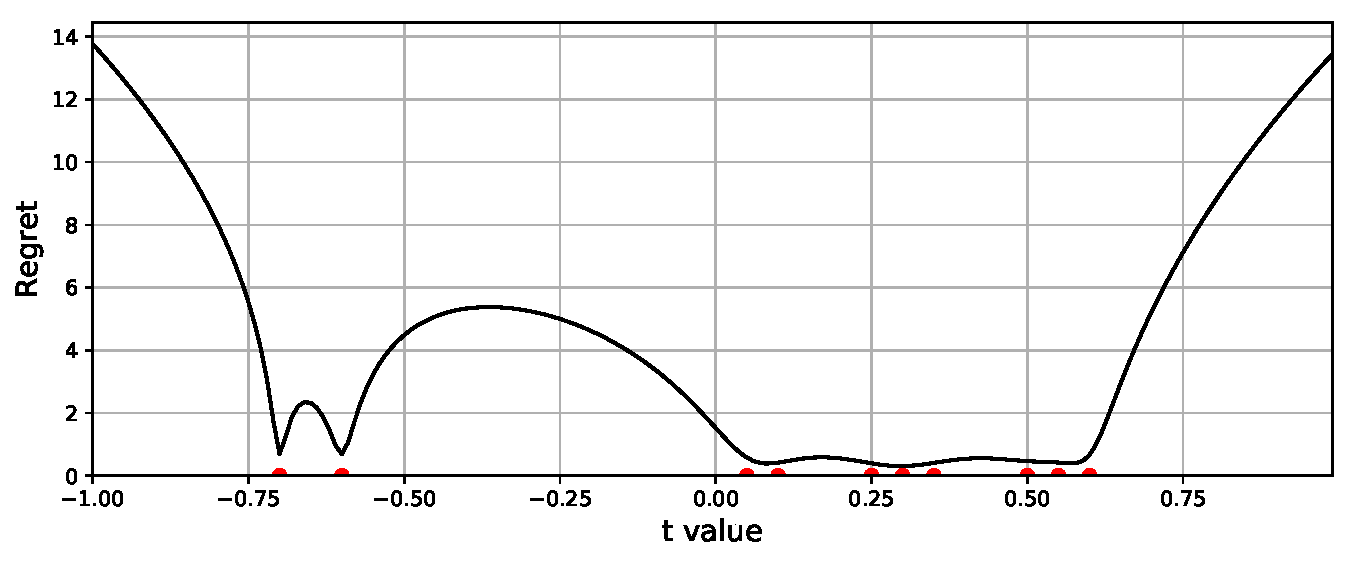
\includegraphics[width=0.6\linewidth]{figures/linear_regression_figures/figure_poly_experiment_regret_10_deg.pdf}
\end{figure}
\end{frame}



\begin{frame}{Simulation with various polynomial degrees}
\begin{figure}
    \vspace{-0.1cm}
    \centering
    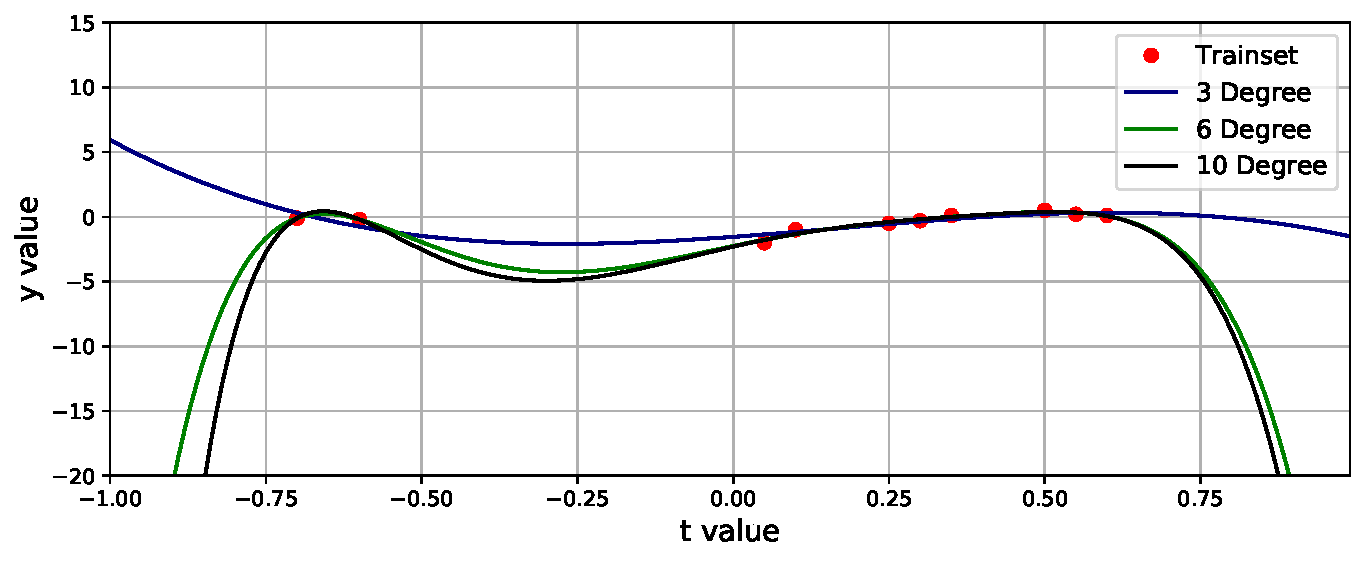
\includegraphics[width=0.6\linewidth]{figure_poly_experiment_prediction_all.pdf}
    \vspace{-0.5cm}
\end{figure}
\pause
\begin{figure}
    \centering
    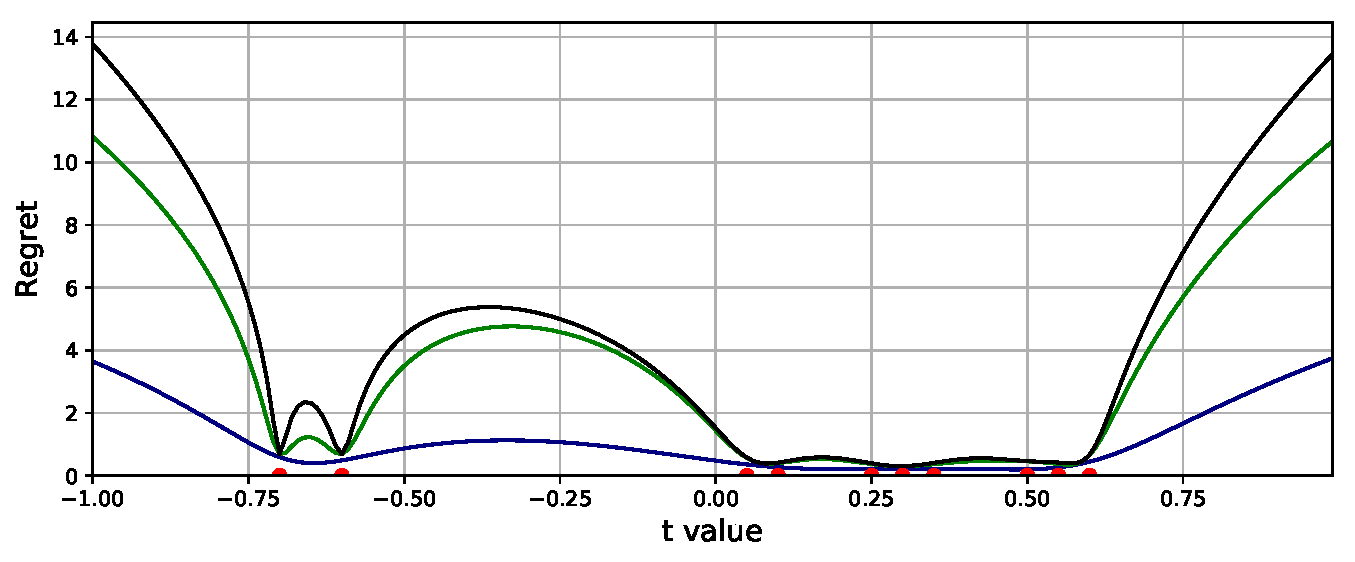
\includegraphics[width=0.6\linewidth]{figure_poly_experiment_regret_all.pdf}
\end{figure}
\end{frame}



% \begin{frame}{Summary}
% \begin{itemize}
%     \item The Universal Learning Setting and pNML Recap
%     \SubItem{Supervised learning in the Individual settings}
%     \SubItem{The pNML attains the minmax regret with respect to the Genie}
%   \vspace{5mm}
%     \pause    
%     \item Analytic solution of the pNML for linear regression was shown
%     \item  The pNML regret
%         \begin{equation*}
%     \Gamma = \log K = \log \left(1 + \frac{1}{N} \sum_{i=0}^{M} \frac{\left(x^\top u_i\right)^2 }{\eta_i}\right)
%         \end{equation*}
%     \item {\bf The ``learnability space'':} Generalization can be attained if the test data mostly lies in a small subspace spanned by eigenvectors of the correlation matrix with large eigenvalues
%     \pause
%     \item Simulations of polynomial fitting 
%  \end{itemize}
% \end{frame}

% ------------------------------ %
\subsection{Deep neural networks}
% ------------------------------ %
\begin{frame}{Deep neural networks}
\begin{itemize}
\setlength\itemsep{2em}
\item DNN is a very rich of the hypothesis class. 
\item State of the art DNNs easily fit a random labeling of the training data~\footfullcite{DBLP:conf/iclr/ZhangBHRV17}
\item We obtain the maximum regret when executing the pNML procedure using DNN
    \begin{equation}
    \Gamma = \log \# \textit{class}
    \end{equation}
\item We propose a method that reduced the richness of the DNN hypothesis class
\end{itemize}
\end{frame}

\begin{frame}{Efficient pNML procedure}
\begin{enumerate}
\item Train a DNN model using the standard ERM training procedure.
\item  Extract the features of the trainset $ \{(\phi(x_i),y_i)\}_{i=1}^N$
\item Add the test instance  $(\phi(x),y)$ to the trainset features with arbitrary choice of $y$
\item Train the single fully connected layer using the ERM procedure
    \begin{equation}
    w_{y} = \argmin_{w} \left[\sum_{i=1}^N  - \log p_{w}\left(y_i|\phi(x_i)\right) 
    - \log p_{w}\left(y|\phi(x)\right) \right].
    \end{equation}
\item Given the trained layer, predict the class it was trained with
\begin{equation}
    p_{y} = p_{w_{y}}(y|\phi(x)).
\end{equation}
\item Repeat 3-5 for every possible label
\item The associated regret is then 
    \begin{equation}
    \Gamma = \log \sum_{y \in \mathcal{Y}} p_{y} 
    = \log \sum_{y \in \mathcal{Y}}  p_{w_{y}}(y|\phi(x)). 
    \end{equation}
\end{enumerate}
\end{frame}


\begin{frame}{The open-set task}
The goal is to simultaneity:
\begin{itemize}
\item classify correctly image with known class
\item alert when image with unknown is presented
\end{itemize}
\centering
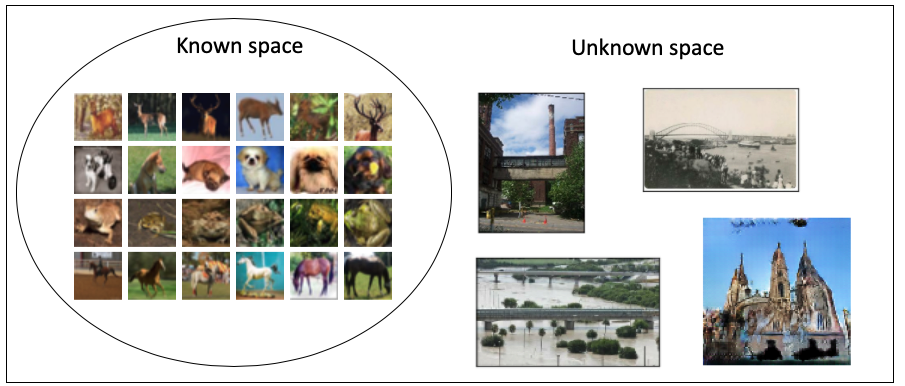
\includegraphics[width=0.7\textwidth]{figures/openset_task.jpg}
\end{frame}


\begin{frame}{Evaluation methodology}
\begin{itemize}
\item  Open-Set Classification Rate (OSCR) evaluation metric
\item  $\mathcal{D}_c$ is a dataset that contains known classes
\item  $S(x)$ is a confidence score for sample x. $T$ is a score threshold, 
\item $c$ is the correct class
\item  The Correct Classification Rate (CCR) 
    \begin{equation}  \label{eq:ccr}
    \mathrm{CCR}(T) = \frac{1}{|\Dc|}\bigl|\{x \mid  x \in \Dc \  \wedge 
    \argmax_{y \in \mathcal{Y}} p(y|x) = c \ \wedge 
    S(x) > T \}\bigr|.
    \end{equation}
\item $\mathcal{D}_u$ contains data with unknowns.
\item The False Positive Rate (FPR)
    \begin{equation}  \label{eq:fpr}
        \mathrm{FPR}(T) =  \frac{1}{|\Du|} \left|\{x \mid x \in \Du \wedge S(x) \geq T \}\right|.
    \end{equation}
\end{itemize}
\blfootnote{Akshay Raj Dhamija et al. ``Reducing Network Agnostophobia'' NIPS 2018}
\end{frame}


\begin{frame}{DNN open-set results}
CCR vs FPR curves of the compared methods with CIFAR10 and CIFAR100  as datasets with known classes. \\
Images from LSUN simulate unexpected inputs. 

\begin{figure}[h]
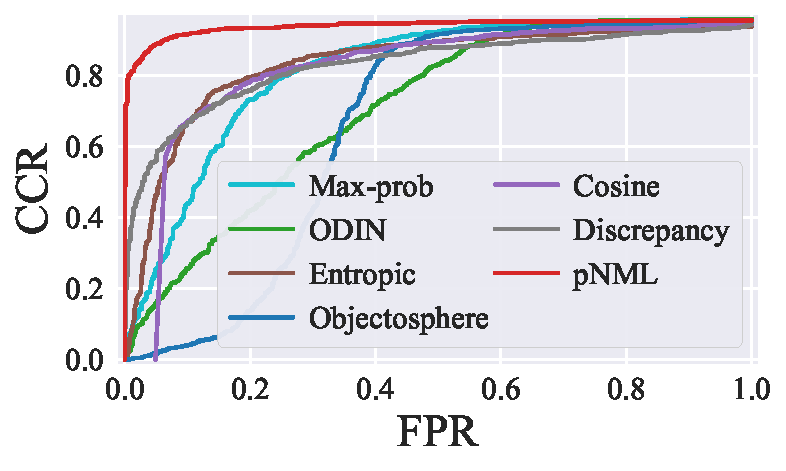
\includegraphics[width=0.45\textwidth]{figures/dnn_openset_figures/figure_pnml_densenet100_cifar10_lsun.pdf}
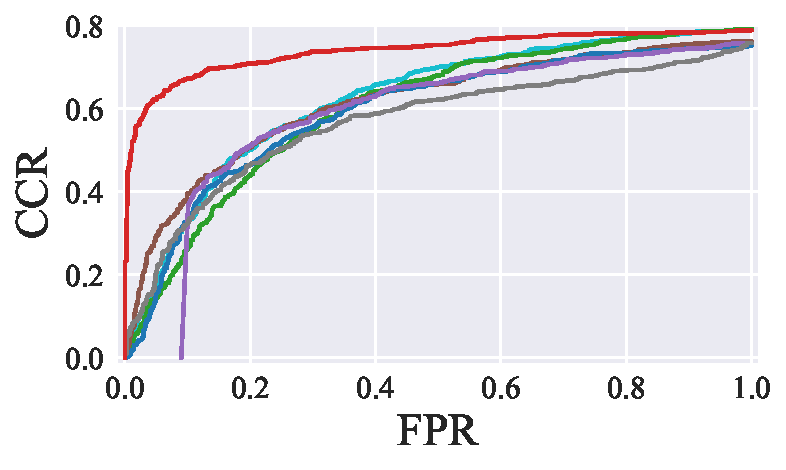
\includegraphics[width=0.45\textwidth]{figures/dnn_openset_figures/figure_pnml_wrn16_cifar100_lsun.pdf}
\end{figure}
More results in \fullcite{pNML_neural_networks}
\end{frame}

\begin{frame}{Hypothesis class experiment}
We consider the following hypothesis class
\vspace{0.25cm}
\begin{enumerate}
\setlength\itemsep{1em}
\item \emph{0 Layers}: Nothing is trained during the fine-tuning phase. This is the ERM learner.
\item \emph{2 Layers}: The fine-tuning alters only the last two layer.
\item \emph{7 Layers}: when the fine-tuning phase affects all layers.
\end{enumerate}
\vspace{0.5cm}
\centering
\begin{tabular}{cccccc}
\toprule
\# Tuned Layers \ \ \ & Acc.  & \ \ Loss avg \ &  \ \ Loss STD \ \ & Regret\\
\hline
0 layers    & 0.920 &  0.203 & 0.87 & 0.0   \\
2 layers    & 0.921 &  0.173 & 0.30 & 0.14  \\
7 layers    & 0.913 &  0.244 & 0.27 & 0.23  \\
\bottomrule
\end{tabular}
\end{frame}

\begin{frame}{Hypothesis class experiment result}
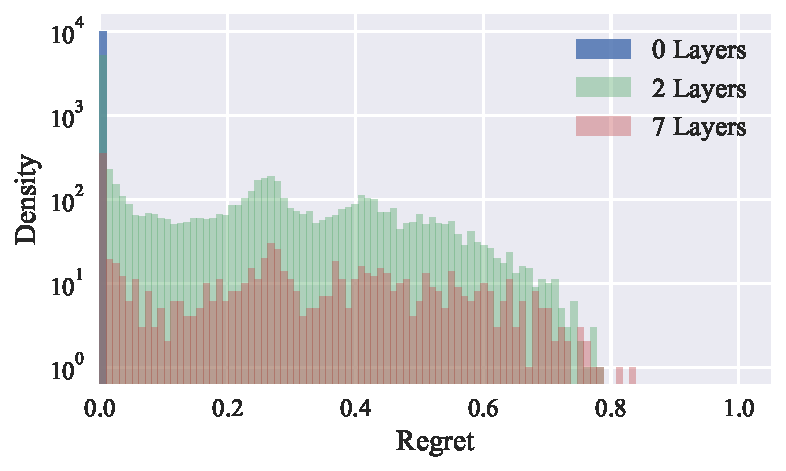
\includegraphics[width=0.49\textwidth]{figures/dnn_openset_figures/figure_resnet18_regret_histogram_num_layers.pdf}
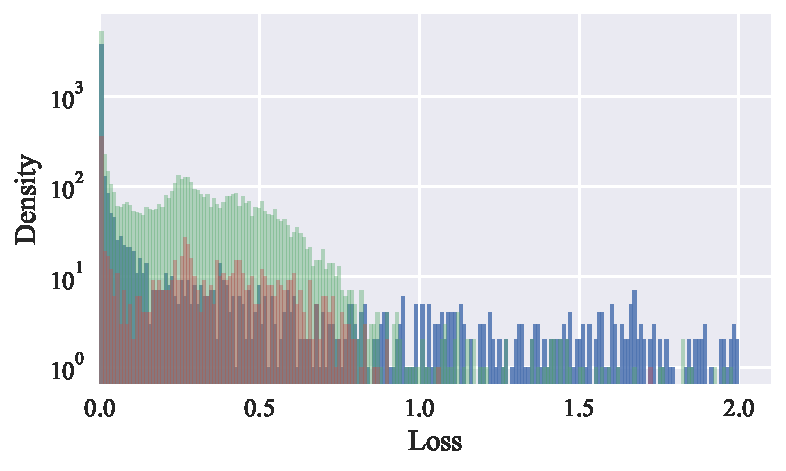
\includegraphics[width=0.49\textwidth]{figures/dnn_openset_figures/figure_resnet18_loss_histogram_num_layers.pdf}
\end{frame}

\begin{frame}{Efficient pNML remarks}
\vspace{-2.0cm}
\begin{itemize}
\setlength\itemsep{2em}
\item We define the hypothesis class as one fully connected layer
\item By using one fully connected layer we are in the undetermined regime
\item Accelerating the pNML procedure
\end{itemize}
\end{frame}

% ------------------------------ %
\section{Future Research}
% ------------------------------ %
\begin{frame}[c]
\begin{center}
\Huge Future Research Directions
\end{center}
\end{frame}

\subsection{Over-parameterized linear regression}
\begin{frame}{Over-parameterized linear regression}
\begin{itemize}
\setlength\itemsep{1.5em}
\item In learning theory is that there should be a trade-off between the training set error and the complexity of the prediction rule.
\item We consider when a perfect fit to training data in linear regression is compatible with an accurate prediction.
\item We plan to focus on the minimum norm solution: the solution that attains a perfect fit on the training set and has the minimum norm than all other solutions that have the perfect fit.
\end{itemize}
\end{frame}



\begin{frame}{Minimum norm linear regression}
Given a training set $z^N =\{(x_i,y_i)\}_{i=1}^N$:
\begin{equation} \label{eq:trainset_matrix}
X_N = 
\begin{bmatrix}
x_1 & x_2 & \dots & x_N
\end{bmatrix}^\top
\in \mathcal{R}^{N \times M},
\quad
Y_N = \begin{bmatrix} y_1 & y_2 & \dots & y_N \end{bmatrix}^\top
\in \mathcal{R}^{N \times 1}.
\end{equation}
The pseudo-inverse of $X_N$ is
\begin{equation} \label{eq:pseudo-inverse}
X_N^+ = 
\begin{cases} 
    (X_N^\top X_N)^{-1} X_N^\top & \textit{Rank}(X_N^\top X_N) = M\\ 
    X_N^\top (X_N X_N^\top )^{-1} & \textit{otherwise} \\   
\end{cases}
\end{equation}
where $X_N^\top X_N \in R^{M \times M}$ and $X_N X_N^\top \in R^{N \times N}$. 
\\
The minimum least squares solution takes the form
\begin{equation}
    \theta_N = X_N^+ Y_N.
\end{equation}
\end{frame}


\begin{frame}{Minimum norm solution norm behaviour}
\begin{theorem}
Denote $||x_\bot||^2 = x^\top \left[I - X_N^\top (X_N X_N^\top )^{-1} X_N \right] x$,
the recursive equation of the norm of the minimum norm solution is given by 
\begin{equation}  \label{eq:mn_solution_norm}
||\theta_{N+1}||^2 = ||\theta_N||^2 + \frac{1}{||x_\bot||^2}(y-x^\top \theta_N)^2.
\end{equation}
\end{theorem}
\end{frame}

\begin{frame}{Minimum norm solution norm behavior}
\begin{itemize}
\setlength\itemsep{1em}
    \item $||x_\bot||^2$ is the projection of the test samples on the training set correlation matrix orthogonal subspace.
    \item If the test sample mostly lies in the subspace of the trainset, $||x_\bot||^2$ becomes small and a slight deviation from the minimum norm prediction increases significantly the norm.
    \item If the test sample lies in the orthogonal subspace, the denominator is relatively large and a deviation from the minimum norm does not change the norm.
    \item For confident prediction, we would like that any other prediction will cause a model with high complexity and therefore we will have high confidence in a prediction in situations where $||x_\bot||^2$ is relatively small.
\end{itemize}
\end{frame}

\begin{frame}{pNML with norm constraint}
\begin{itemize}
\item  The hypothesis set contains learners that have a norm that is smaller or equals to the norm of the minimum norm solution.
\item For each possible test label we wish to find its corresponding regularization factor $\lambda$ that satisfies the equation
$||\hat{\theta}(z^N,x,y,\lambda)||^2 = ||\theta_{MN}||^2$ 
\item Notice that $\lambda$ depends on $y$
\item Compute the normalization factor
    \begin{equation}
    K
    = 
    \int_{-\infty}^\infty
    \frac{1}{\sqrt{2 \pi \sigma^2}} \exp \left\{-
    \frac{\left(y- x^\top \hat{\theta}(z^N,x,y,\lambda) \right)^2}{2 \sigma^2} \right\} dy.
    \end{equation}
\end{itemize}
\end{frame}

\begin{frame}{pNML with norm constraint simulation}
\begin{itemize}
\item The training set consist of 4 points $\{(t_i,y_i)\}_{i=1}^4$ in the interval $[-1, 1]$
\item The relation between $y$ and $t$ using the Fourier base
    \begin{equation}
    X_{N}[i,m]
    =
    \sqrt{\pi} \cos \left(\pi m t_i +  \frac{\pi}{2} m\right) .
    \end{equation}
\end{itemize}

\centering
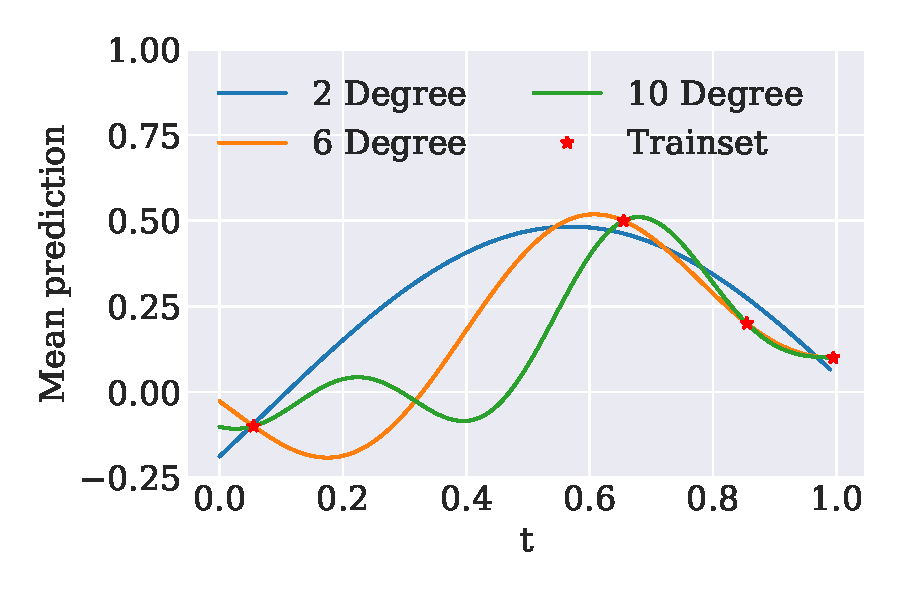
\includegraphics[width=0.49\textwidth]{figures/overparam_pnml_linear_regression/figure_pnml_linear_regression_mn_prediction.pdf}
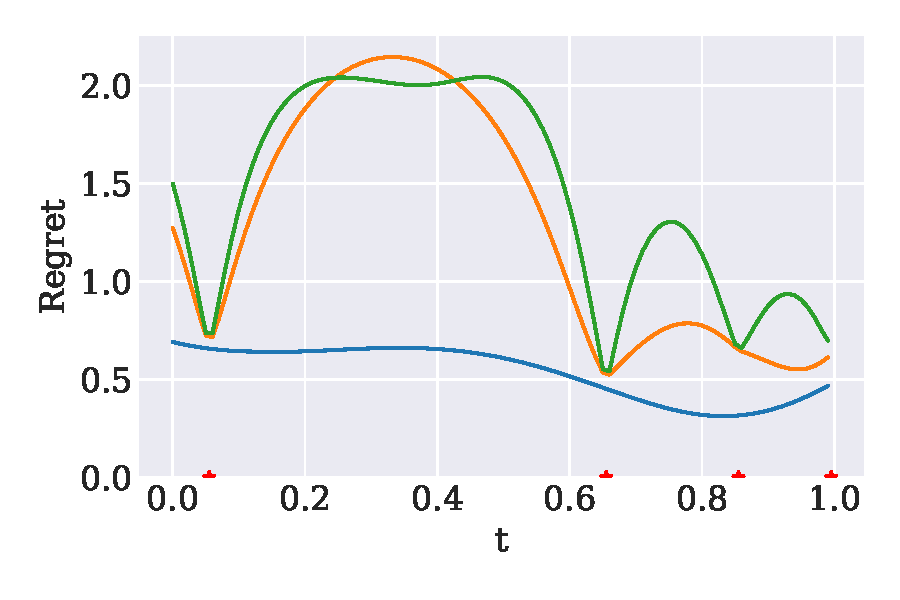
\includegraphics[width=0.49\textwidth]{figures/overparam_pnml_linear_regression/figure_pnml_linear_regression_mn_regret.pdf}
\end{frame}

\subsection{Logistic regression}
\begin{frame}{Logistic regression}
\begin{itemize}
\item A statistical model that uses a logistic function to model a binary dependent variable.
\item The model maps a test feature into binary class.
\item Denote $w$ as the learnable parameters, the probabilities of a test feature $x$ to have label '0' and '1' are:
\begin{equation}
    p(y=0|x,z^N) = \frac{e^{-w^\top x}}{1 + e^{-w^\top x}} = \frac{1}{1 + e^{w^\top x}}, \qquad
    p(y=1|x, z^N) = \frac{1}{1 + e^{-w^\top x}}.
\end{equation}
\item The ERM solution $w_N$ is usually obtained by minimizing the training log-loss using optimization techniques such as gradient descent
\begin{equation}
w_N = \argmin_{w} \left[ - \sum_{i=1}^N \log p(y_i|x_i) \right].
\end{equation}
\end{itemize}
\end{frame}

\begin{frame}{Logistic regression recursive solution}
\begin{itemize}
\item A recursive form of logistic regression using the linear regression minimum norm solution was recently suggested~\footfullcite{zhuang2020training}.
\item Denote $f(\cdot)$ as the activation function, 
\begin{equation}
    g = \left(x^\top \left(I - X^+_N X_N \right) \right)^+, \quad  z = f^{-1}(y),
\end{equation}
\item The recursive logistic regression formula is
\begin{equation} \label{eq:logistig_regression_recurisve}
    w_{N+1} = w_N + g \left(z - x^\top w_N \right).
\end{equation}
\end{itemize}
\end{frame}

\begin{frame}{Logistic regression pNML}
\begin{itemize}
\item The log normalization factor is the pNML regret:
\begin{equation}
    \log K = \log \left(p_{\hat{\theta}(z^N,x,y=0)}(y=0|x) + p_{\hat{\theta}(z^N,x,y=1)}(y=1|x)\right).
\end{equation}
\item Initial results show that the pNML regret using the recursive update rule is
\begin{equation}
    \Gamma = \log K = \log \left(1 + \frac{1}{1 +  \mathbf{1}_{||x_\bot|| = 0} \left[ 2\cosh{\left(x^\top w_N \right)} \right]}\right).
\end{equation}
\item If the test sample fully lies in the trainset subspace: $||x_\bot||=0$ and the regret is
\begin{equation}
\Gamma = \log \left(1 + \frac{1}{1 + 2\cosh{\left(x^\top w_N \right)}}\right).
\end{equation}
The regret is bounded by $0 \leq \Gamma \leq 1\frac{1}{3}$.
\item If there is a portion of the test sample that lies in the trainset orthogonal subspace, $||x_\bot||>0$ and the maximal possible regret is obtained.
\end{itemize}
\end{frame}

\begin{frame}{Logistic regression future research}
\begin{itemize}
\setlength\itemsep{2em}
    \item Compare the regret of the recursive solution and the gradient descent based solution.
    \item  Use this recursive method with the open-set classification task for accelerating the compute time of the pNML.
    \item Develop the pNML regret for logistic regression with gradient decent.
\end{itemize}
\end{frame}

\subsection{DNN}
\begin{frame}{DNN future research}
Complexity constraint
\begin{itemize}
\item Using DNN, the model fits exactly to each possible test label. 
Using the regret as a generalization measure might be useless.
\item We introduced the pNML with norm constraint. We can apply a similar approach for DNN: Find a property that defines the complexity of the DNN model and use it to constrain the pNML learner.
\item Researchers have proposed many ways to quantify the complexity of DNN models: the number of degrees of freedom~\footfullcite{gao2016degrees}, prequential code~\footfullcite{blier2018description} and intrinsic dimension~\footfullcite{li2018measuring}.
Using these methods as a constraint in the pNML scheme might lead to a meaningful regret.
\end{itemize}
\end{frame}



\begin{frame}
\Huge{\centerline{The End}}
\end{frame}


% ------------------------------ %
% Appendix
% ------------------------------ %
\backupbegin
\begin{frame}[c]
\begin{center}
\Huge Appendix
\end{center}
\end{frame}

\begin{frame}{pNML Proof}
    
\end{frame}


\begin{frame}{Open-set competitors}
\begin{itemize}
\item Max-prob: \\ \fullcite{hendrycks2016baseline}
\item ODIN: \\ \fullcite{liang2017enhancing}
\item Entropic open-set, Objectosphere: \\ \fullcite{dhamija2018reducing}
\item Cosine Similarity: \\ \fullcite{wang2018cosface}
\item Maximum Discrepancy: \\ \fullcite{yu2019unsupervised}
\end{itemize}
\end{frame}
\begin{frame}{Open-set competitors}
\begin{itemize}
\item Max-prob: \\ \fullcite{hendrycks2016baseline}
\item ODIN: \\ \fullcite{liang2017enhancing}
\item Entropic open-set, Objectosphere: \\ \fullcite{dhamija2018reducing}
\item Cosine Similarity: \\ \fullcite{wang2018cosface}
\item Maximum Discrepancy: \\ \fullcite{yu2019unsupervised}
\end{itemize}
\end{frame}


\backupend
\end{document}

